
% Preamble

\documentclass[11pt]{article}

% Packages
\usepackage{amsmath}
\usepackage{mathtools}
\usepackage{ragged2e}
\usepackage [utf8]{inputenc}
\usepackage{blindtext}
\usepackage{wrapfig}
\usepackage{xcolor}
\usepackage {polski}
\usepackage{multicol}
\usepackage[a4paper, total={5.7in, 8in}]{geometry}
\usepackage{graphicx}
\usepackage{amstex}
\usepackage{csvsimple}
\usepackage{changepage}
\usepackage{enumitem}
\usepackage[english]{babel}
\usepackage{biblatex}
\usepackage{caption}
\usepackage{indentfirst}
\usepackage{epstopdf-base}
\usepackage{textcomp}
\usepackage{wasysym}

% Document
\begin{document}
%    Nagłówek
    \begin{flushleft}
        Maciej Pierzchała 282 934 \hfill Data wykonania ćwiczenia:\\
        Filip Kubecki 272 655 \hfill 3 grudnia 2024r\\
        Grupa: Wtorek 10:35 \\
    \end{flushleft}
    \vspace{1cm}
    \begin{center}
        \Large\textbf{Laboratorium 8}\\
        \textbf{Charakteryzacja czujnika zbliżeniowego}
    \end{center}
    \hfill
    \vspace{4cm}
%    Treść
    \section{Spis przyrządów}
    \par{
        Do wykonania ćwiczenia wykorzystano:
        \begin{itemize}
            \setlength\itemsep{0em}
            \item[-] Zasilacz labolatoryjny
            \item[-] Laserowy czujnik odległości OM70-11112064
            \item[-] Laserowy czujnik odległości OT500.DL-GLIAJ.72F
            \item[-] Ultradźwiękowy czujnik odległości U500.DA0-11126857
            \item[-] Próbki różnych powierzchni (do badania odbicia)
        \end{itemize}
    }
    \section{Przebieg i cele doświadczenia}
    \par Ćwiczenie polegało na badaniu zachowań trzech różnych czujników zbliżeniowych na różne powierzchnie odbicia.
    W cyklu ćwiczenia zapoznawano się również ze zmianą zachowania czujnika ultradźwiękowego zależnie od trybu pracy.\\
%    \section{Kluczowe parametry sensorów}
%    \subsection{OT500.DL-GLIAJ.72F}
%    Measuring distance: 150\dots 2500[mm]\\
%    Beam type: point\\
%    Light source: pulsed red laser diode\\
%    Wave length: 680[nm]
%    Response time:\\
%    - 4 ms - High Speed Mode\\
%    - 8 ms - Standard Mode\\
%    - 50 ms - Long Range Mode\\


    \section{Analiza wyników}
    \noindent\makebox[\textwidth]{
        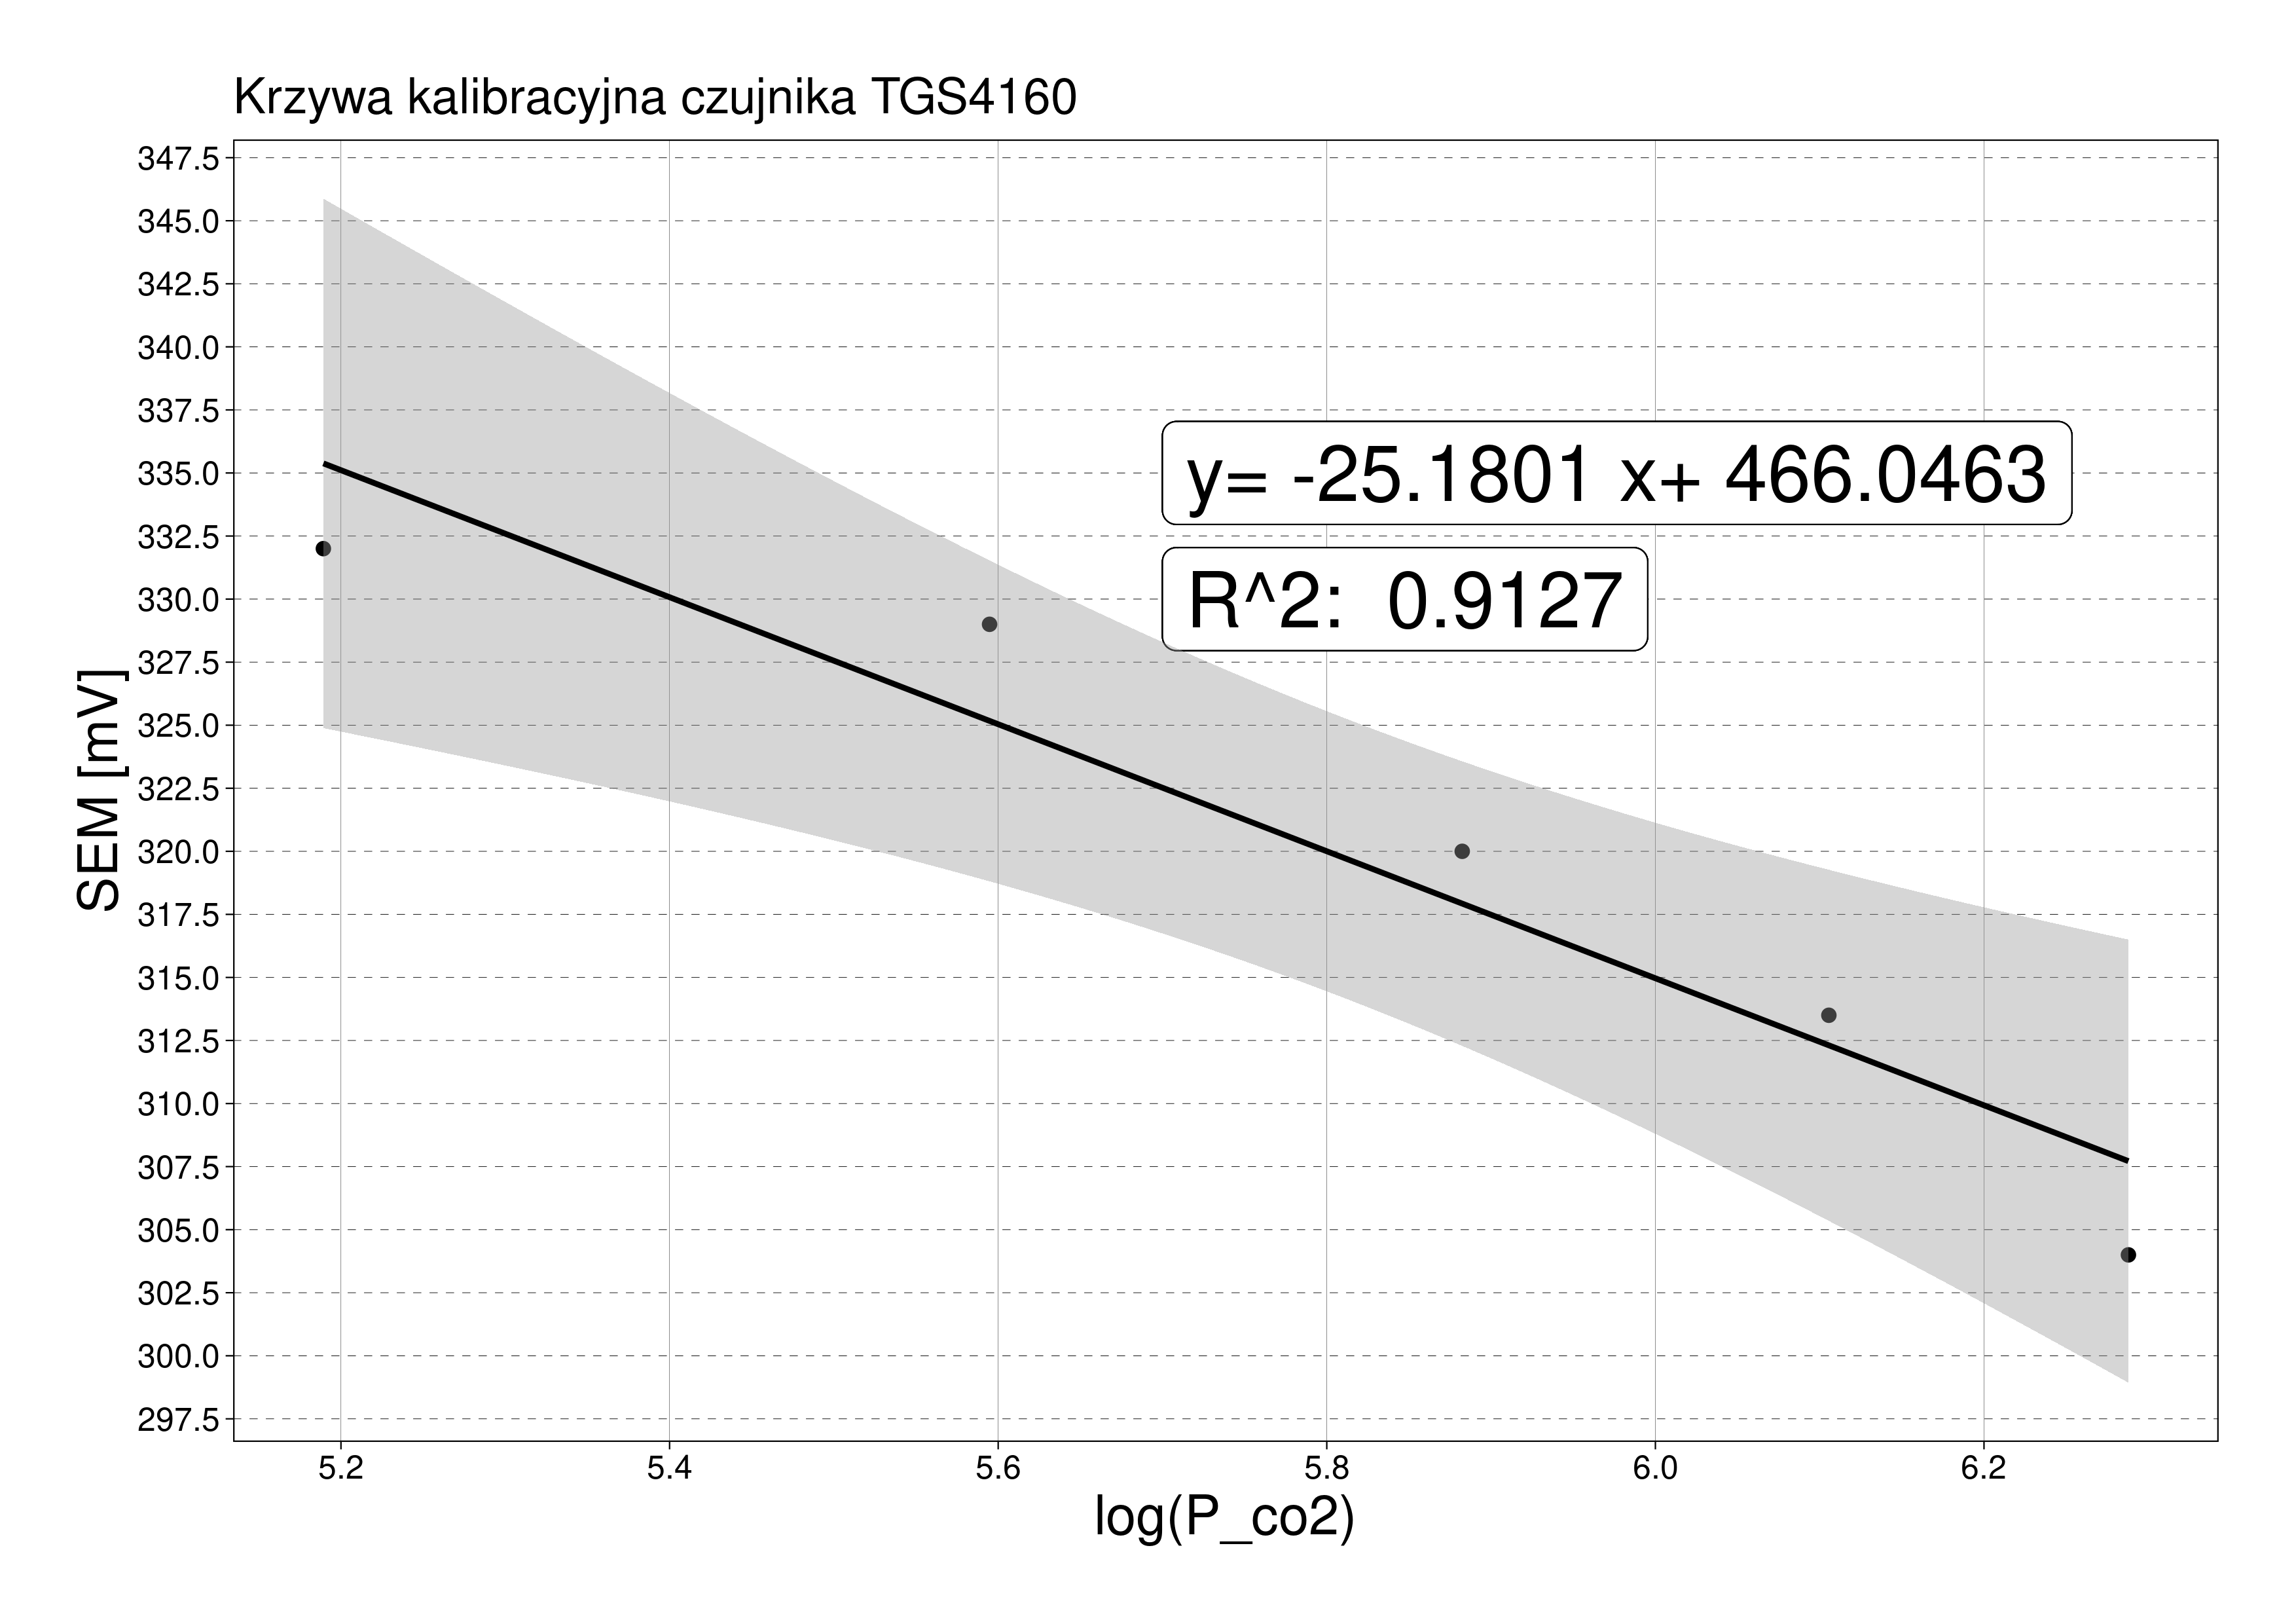
\includegraphics[scale = 0.6]{/home/bork/IdeaProjects/LatexProjects/src/PodstawyTechnikiSensorowej/Lab8/Img/plot1}}
    \indent Gdzie:
        {\footnotesize
    \begin{itemize}
        \setlength\itemsep{0em}
        \item[] \textbf{$\otimes$} - tryb wide
        \item[] \textbf{$\bigcirc$} - tryb narrow
        \item[] \textbf{$\triangle$} - tryb medium
    \end{itemize}}

    \subsection{Tabela 1 - czujnik ultradźwiękowy, szerokość zależnie od trybu}
    \begin{center}
        \Large\csvreader[tabular = |c|c|c|c|,
            table head = \hline  \textbf{Dystans[cm]}  & \textbf{Narrow[cm]} & \textbf{Medium[cm]} & \textbf{Wide[cm]}  \\\hline,
            late after line = \\\hline
        ]{Data/data.csv}{}{
            \csvcoli & \csvcolii & \csvcoliii & \csvcoliv
        }
    \end{center}
    \subsection{Tabela 2 - wykrywanie różnych rodzajów materiałów}
    \begin{center}
        \Large\csvreader[tabular = |c|c|c|c|,
            table head = \hline  \textbf{Materiał}  & \textbf{U500[cm]} & \textbf{OM70[cm]} & \textbf{OT500[cm]}  \\\hline,
            late after line = \\\hline
        ]{Data/dataReflect.csv}{}{
            \csvcoli & \csvcolii & \csvcoliii & \csvcoliv
        }
    \end{center}
    \section{Wnioski}
    \par Na podstawie pierwszego badania zależności szerokości pola wykrywania czujnika ultradźwiękowego zależnie od trybu
    pracy można zauważyć odpowiednie odwzorowanie szerokości pola od trybu. Ze wzrostem odległości szerokość wykrywania
    rosła co zgadza się z przewidywanym działaniem czujnika. Również szerokość pola wykrywania była odpowiednia względem
    trybu pracy. Najwęższe pole otrzymaliśmy dla trybu "narrow" a najszersze dla trybu "wide".\\
    \indent Na podstawie wyników z badania reakcji czujników na różne powierzchnie odbijające zauważono że czujniki nie miały problemu
    z wykrywaniem większości powierzchni. Jedyne odejścia od normy zaobserwowano dla czujnika optycznego OT500 dla pomiarów "odbłyśnika" oraz
    przy podstawieniu na odległości 10[cm] szkiełka labolatoryjnego. Dla "odbłyśnika" czujnik zarejestrował wartość o 10[cm] za dużą. Ciężko jednak
    stwierdzić czy to rzeczywisty błąd czujnika czy błąd mierzącego dlatego pomiar ten uznajemy dla pewności za błędny. Inaczej się ma pomiar
    ze szkiełkiem labolatoryjnym włożonym na odległości 10[cm] przez właściwą powierzchnią odbijającą. Czujnik ten niezarejestrował przeszkody
    na dystansie 10[cm] tylko kolejną na odległości 40[cm]. Wynika to prawdopodobnie z zakresu pracy tego czujnika którego zakres wykrywania
    przedstawiony w nocie katalogowej zaczyna się od odległości 15[cm]. Zakresy pomiarowe pozostałych czujników zaczynają się za to od odległości
    10[cm] co tłumaczy dlaczego wykryły one pierwszą przeszkodę.\\
    \indent Odpowiadając jeszcze na pytanie jaki czujnik byłby najlepszym wyborem jako czujnik parkowania najlepszą odpowiedzią byłby czujnik
    OT500. Pracuje on na zakresie odległości 15 - 250 [cm] co jest dość optymalnym zakresem dla odległości parkowania. Dla idealnego działania
    dobrym zasotowaniem byłby jednak ukłąd hybrydowy składający się z czujnika OT500 oraz ultradźwiękowego czujnia U500 ustawionego na tryb medium lub
    wide. Miałby to na celu wykrywanie przeszkód które zbudowane są w sposób nieciągłby np.: siatki, płoty.



    %Bibliografia
    \vfill
    \footnotesize
    \begin{thebibliography}{3}
        \bibitem{texbook1}
        https://docs.rs-online.com/ac70/A700000009505302.pdf
        \bibitem{texbook2}
        https://www.baumer.com/medias/\_\_secure\_\_/Baumer\_OM70-P0600.HH0500.VI\\ \_EN\_20201216\_DS.pdf?mediaPK=9009237393438
        \bibitem{texbook3}
        https://www.baumer.com/medias/\_\_secure\_\_/U500\_DA0\_UA1B\_72O0\_0000\_web\_EN.pdf?mediaPK=8800549634078
    \end{thebibliography}
\end{document}
}